\section{Complete current result tables}

\begin{table}[h]
\caption{Five-seed GAR ablations on stylized iGSM.}
\label{tab:ablations}
\centering
\small
\begin{tabular}{lcc}
\toprule
Variant & Strict & $+2$ actions \\
\midrule
Full GAR & $.433\pm.019$ & $.796\pm.033$ \\
No GAR & $.076\pm.013$ & $.422\pm.022$ \\
Latent MSE only & $.183\pm.016$ & $.628\pm.031$ \\
Ranking only & $.358\pm.045$ & $.750\pm.018$ \\
No counterfactual latent loss & $.345\pm.049$ & $.734\pm.017$ \\
GAR horizon 1 & $.161\pm.021$ & $.597\pm.037$ \\
GAR horizon 2 & $.433\pm.019$ & $.796\pm.033$ \\
GAR horizon 4 & $.181\pm.008$ & $.651\pm.014$ \\
One counterfactual & $.403\pm.041$ & $.772\pm.020$ \\
Four counterfactuals & $.439\pm.049$ & $.821\pm.025$ \\
Advantage MSE weight $.10$ & $.443\pm.037$ & $.802\pm.034$ \\
Advantage MSE weight $.50$ & $.402\pm.039$ & $.783\pm.026$ \\
\bottomrule
\end{tabular}
\end{table}

\begin{table}[h]
\caption{One-seed mechanism controls. These rows are exploratory. Geometry-only uses an oracle-terminal embedding and is candidate privileged.}
\label{tab:mechanism}
\centering
\small
\begin{tabular}{lcc}
\toprule
Variant & Strict & $+2$ actions \\
\midrule
Full GAR & $.435$ & $.820$ \\
Detached GAR body & $.375$ & $.775$ \\
GAR without counterfactual latent loss & $.255$ & $.695$ \\
Counterfactual latent only & $.080$ & $.410$ \\
Direct ranker with successor auxiliaries & $.440$ & $.820$ \\
Raw geometry only\privileged & $.190$ & $.625$ \\
\bottomrule
\end{tabular}
\end{table}

\begin{table}[h]
\caption{Five-seed representation diagnostics. Probe values are means across seeds.}
\label{tab:probes}
\centering
\scriptsize
\begin{tabular}{lrrrrr}
\toprule
Model & Effective rank & Operation bal. acc. & Remaining $R^2$ & Resolved $R^2$ & Outcome $R^2$ \\
\midrule
MLP JEPA & $198.70$ & $.406$ & $.346$ & $.895$ & $.088$ \\
Causal JEPA & $215.34$ & $.403$ & $.332$ & $.846$ & $.053$ \\
Token LM & $3.55$ & $.532$ & $.439$ & $.986$ & $-.020$ \\
Sentence LM & $79.64$ & $.777$ & $.410$ & $.879$ & $-.027$ \\
Sentence LM + latent & $71.44$ & $.807$ & $.429$ & $.886$ & $-.029$ \\
\bottomrule
\end{tabular}
\end{table}

\begin{table}[h]
\caption{One-seed information controls across a local learning-rate screen. These controls separate meaningful counterfactual ordering from counterfactual exposure alone.}
\label{tab:information-controls}
\centering
\small
\begin{tabular}{lccc}
\toprule
Control & Learning rate & Strict & $+2$ actions \\
\midrule
Direct ranker without successor auxiliaries & $10^{-4}$ & $.180$ & $.590$ \\
Direct ranker without successor auxiliaries & $3\times10^{-4}$ & $.185$ & $.635$ \\
Direct ranker without successor auxiliaries & $7\times10^{-4}$ & $.150$ & $.560$ \\
GAR with shuffled quality labels & $10^{-4}$ & $.015$ & $.170$ \\
GAR with shuffled quality labels & $3\times10^{-4}$ & $.015$ & $.175$ \\
GAR with shuffled quality labels & $7\times10^{-4}$ & $.015$ & $.175$ \\
\bottomrule
\end{tabular}
\end{table}

\begin{table}[h]
\caption{Exploratory recurrent-depth language-model curves. These are raw one-seed loop results. FLOP calibration under fixed candidate work is pending.}
\label{tab:looped}
\centering
\scriptsize
\begin{tabular}{llrrrrrr}
\toprule
Model & Metric & 1 loop & 2 loops & 4 loops & 8 loops & 16 loops & 32 loops \\
\midrule
Token LM & Strict & $.065$ & $.140$ & $.155$ & $.170$ & $.170$ & $.140$ \\
Token LM & $+2$ & $.550$ & $.700$ & $.705$ & $.725$ & $.695$ & $.650$ \\
Sentence LM & Strict & $.290$ & $.430$ & $.475$ & $.450$ & $.395$ & \todoresult \\
Sentence LM & $+2$ & $.700$ & $.800$ & $.800$ & $.740$ & $.735$ & \todoresult \\
Sentence LM + latent & Strict & $.315$ & $.340$ & $.360$ & $.385$ & $.355$ & \todoresult \\
Sentence LM + latent & $+2$ & $.705$ & $.770$ & $.770$ & $.795$ & $.785$ & \todoresult \\
\bottomrule
\end{tabular}
\end{table}

\begin{table}[h]
\caption{Leakage-free one-seed scaling gate on 1,000 paired episodes. Depth greater than one uses a candidate-privileged future action tree.}
\label{tab:scaling-gate}
\centering
\small
\begin{tabular}{lrrr}
\toprule
Score & Depth 1 & Depth 2 & Depth 4 \\
\midrule
JEPA + GAR & $.471$ & $.106$ & $.135$ \\
Direct ranker with successor auxiliaries & $.432$ & $.122$ & $.085$ \\
Zero score & $.068$ & $.078$ & $.076$ \\
Shuffled JEPA score & $.071$ & $.075$ & $.070$ \\
Exact symbolic transition + direct score\privileged & $.432$ & $.141$ & $.087$ \\
\bottomrule
\end{tabular}
\end{table}

\begin{figure}[h]
\centering
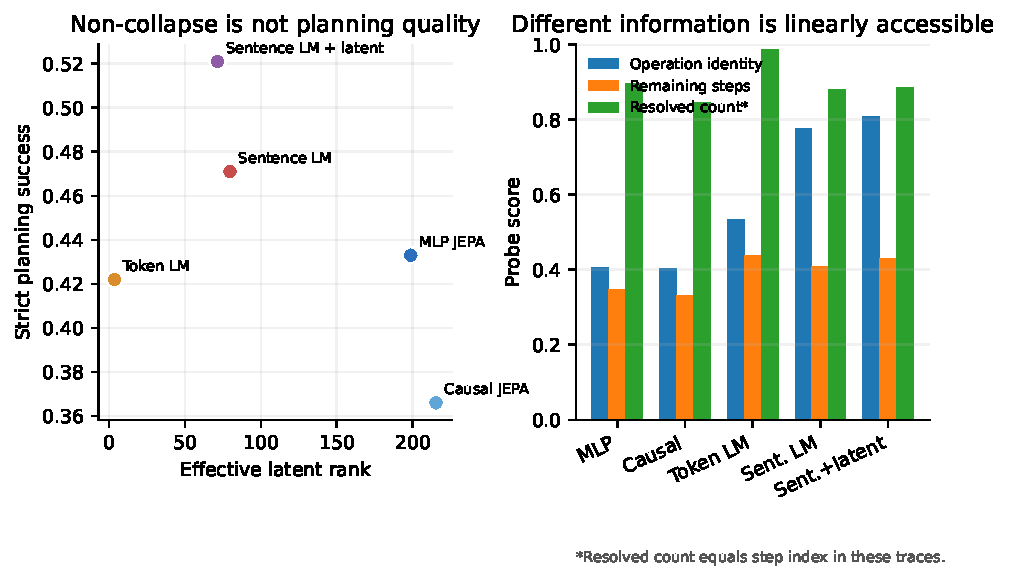
\includegraphics[width=\linewidth]{figures/representation_diagnostics.pdf}
\caption{Five-seed frozen-feature diagnostics. Effective rank is not aligned with planning success. Sentence objectives make operation identity more accessible, while all systems expose progress-related variables. Resolved count remains confounded with elapsed step index.}
\label{fig:representations}
\end{figure}

\begin{table}[h]
\caption{Paper-suite completion matrix. Empty entries are intentional.}
\label{tab:completion}
\centering
\small
\begin{tabular}{lcccc}
\toprule
Experiment family & Stylized iGSM & Faithful iGSM & ProofWriter & Blocksworld / ALFWorld \\
\midrule
Five-seed headline & complete & \todoresult & \todoresult & \todoresult \\
Five-seed GAR ablation & complete & \todoresult & \todoresult & \todoresult \\
Local ordering audit & one seed & \todoresult & \todoresult & \todoresult \\
Length OOD & partial & \todoresult & \todoresult & \todoresult \\
Controlled minimal pairs & \todoresult & \todoresult & \todoresult & \todoresult \\
Test-time FLOP scaling & repaired pilot & \todoresult & \todoresult & \todoresult \\
\bottomrule
\end{tabular}
\end{table}
